\nonstopmode % halt on errors
\documentclass[onecolumn, draftclsnofoot,10pt, compsoc]{IEEEtran}
\usepackage{graphicx}
\usepackage{url}
\usepackage{setspace}

\usepackage{geometry}
\geometry{textheight=9.5in, textwidth=7in}

% 1. Fill in these details
\def \CapstoneTeamName{		The Secret Bunny Team}
\def \CapstoneTeamNumber{		38}
\def \GroupMemberOne{			Andrew Ekstedt}
\def \GroupMemberTwo{			Scott Merrill}
\def \GroupMemberThree{			Scott Russell}
\def \CapstoneProjectName{		Privacy Preserving Cloud, Email, and Password Systems}
\def \CapstoneSponsorCompany{	OSU}
\def \CapstoneSponsorPerson{		Attila Yavuz}

% 2. Uncomment the appropriate line below so that the document type works
\def \DocType{	%Problem Statement
				%Requirements Document
				%Technology Review
				Design Document
				%Progress Report
				}

\newcommand{\NameSigPair}[1]{\par
\makebox[2.75in][r]{#1} \hfil 	\makebox[3.25in]{\makebox[2.25in]{\hrulefill} \hfill		\makebox[.75in]{\hrulefill}}
\par\vspace{-12pt} \textit{\tiny\noindent
\makebox[2.75in]{} \hfil		\makebox[3.25in]{\makebox[2.25in][r]{Signature} \hfill	\makebox[.75in][r]{Date}}}}
% 3. If the document is not to be signed, uncomment the RENEWcommand below
%\renewcommand{\NameSigPair}[1]{#1}

%%%%%%%%%%%%%%%%%%%%%%%%%%%%%%%%%%%%%%%
\begin{document}
\begin{titlepage}
    \pagenumbering{gobble}
    \begin{singlespace}
        %\includegraphics[height=4cm]{coe_v_spot1}
        \hfill
        % 4. If you have a logo, use this includegraphics command to put it on the coversheet.
        %\includegraphics[height=4cm]{CompanyLogo}
        \par\vspace{.2in}
        \centering
        \scshape{
            \huge CS Capstone \DocType \par
            {\huge Rough draft}\par % TODO remove this line
            {\large\today}\par
            \vspace{.5in}
            \textbf{\Huge\CapstoneProjectName}\par
            \vfill
            {\large Prepared for}\par
            \Huge \CapstoneSponsorCompany\par
            \vspace{5pt}
            {\Large\NameSigPair{\CapstoneSponsorPerson}\par}
            {\large Prepared by }\par
            Group\CapstoneTeamNumber\par
            % 5. comment out the line below this one if you do not wish to name your team
            \CapstoneTeamName\par
            \vspace{5pt}
            {\Large
                \NameSigPair{\GroupMemberOne}\par
                \NameSigPair{\GroupMemberTwo}\par
                \NameSigPair{\GroupMemberThree}\par
            }
            \vspace{20pt}
        }
        \begin{abstract}
        % 6. Scott Russell
		 This document explores our implementation with a focus on looking at the exact timeline of implimentation by flushing out the Gantt chart's timeline into more clear and consice week by week evaluations. The points of design for this document include's the searchable encrpytion algorithm, Research of parallelization, and Benchmarking comparisons between other similar algorithm implementations. Each of these major sections contain sub parts that pertain to specific problems we may run into during implementation and how we plan to overcome said problems.
        \end{abstract}
    \end{singlespace}
\end{titlepage}
\newpage
\pagenumbering{arabic}
\tableofcontents
% 7. uncomment this (if applicable). Consider adding a page break.
\listoffigures
%\listoftables
\clearpage

% IEEE Std 1016-2009 § 4.1
% The required contents of an SDD are as follows:
% ⎯ Identification of the SDD
% ⎯ Identified design stakeholders
% ⎯ Identified design concerns
% ⎯ Selected design viewpoints, each with type definitions of its allowed design elements and design languages
% ⎯ Design views
% ⎯ Design overlays
% ⎯ Design rationale

% IEEE Std 1016-2009 § Annex C
% Example outline for a design doc:
%
% Frontspiece
%	Date of issue and status
%	Issuing organization
%	Authorship
%	Change history
% Introduction
%	Purpose
%	Scope
%	Context
%	Summary
% References
% Glossary
% Body
%	Identified stakeholders and design concerns
%	Design viewpoint 1
%	Design view 1
%	...
%	Design viewpoint n
% 	Design view n
% 	Design rationale

\section{Introduction}

\subsection{ Purpose }

The purpose of this document is to specify the system design for the Privacy Preserving Cloud project, and to give an estimated schedule.

\subsection{ Scope }



\subsection{ Context }



\subsection{ Summary }

% XXX References?

\section{ Definitions }

\paragraph*{\textbf{searchable encryption scheme}} An algorithm which allows a client to efficiently search encrypted documents on a remote server.

\paragraph*{\textbf{Parallelize}} adapt (a program) for running on a parallel processing system.
% etc


% Design concerns / constrains

% From the assignment description:
% > In the design document each member will write up the design of each of the three pieces he/she will be owning and managing for the remainder of the year. The entire group will then combine individual work into one full document, framed with a proper introduction and conclusion. You will be graded as a group as you were with the requirements document.
% > This document should include the full *HOW* of your system including your API, your timeline, necessary testing information, etc. Use this document as a guide to plan the rest of the year's work. Remember, a week of debugging can save you 20 minutes of planning! Plan the work, work the plan.


\section{ Project components }

AE will be primarily responsible for \ref{subsec:sse} and \ref{subsec:dumbserver}.
SM will be primarily responsible for \ref{subsec:parallel} and \ref{subsec:size}.
SR will be primarily responsible for \ref{subsec:email} and \ref{subsec:benchmark}.

% Something about being a research-focused project

\subsection{ Searchable encryption algorithm }
\label{subsec:sse}

% Andrew Ekstedt

% gonnna do cash

% - written in C++
% - operations: search, update, delete
% - using tomcrypt for crypto primitives
% - using AES-128-CTR for encryption scheme
% - using HMAC-SHA1 for variable-length PRF(?)
% - using ZeroMQ for client-server communication

The heart of our project is the searchable encryption algorithm. We plan to implement the algorithm described in \cite{cash14}.

There are 3 subcomponents to this component.

\subsubsection{ Search algorithm }

The core subcomponent is C++ library which implements the SSE algorithm.

Search operations:
% XXX these operations should have a server half and client half
\begin{itemize}
\item \textbf{Gen} generates a secret key
\item \textbf{Setup} constructs an encrypted search index from an initial set of files
\item \textbf{Search} takes a search keyword and returns a list of matching files
\item \textbf{Update} takes an operation (add, delete), a file id, and a list of keywords and performs the appropriate action
\end{itemize}

Cash DSSE relies on two cryptographic primitives: a symmetric encryption scheme and a variable-length input PRF. We plan to use AES-128-CTR for the encryption scheme and HMAC-SHA256 for the PRF. Implementations of both algorithms will be supplied by the tomcrypt \cite{tomcrypt} library.

\subsubsection{ Server program }

The server program is a daemon which responds to client requests.
The client and server will exchange messages with the ZeroMQ library.
The server is responsible for maintaining the encrypted files and encrypted search index.

Encrypted files will be stored on the remote filesystem in a flat directory structure. When the client requests a file, the encrypted copy will be sent to the client and decrypted on the client side.
%- how to store files

The index will be stored as a file in an ad-hoc format. Cash DSSE combines several data structures--the main search index, which is static, and two smaller data structures to keep track of additions and deletions. We can store these different data structures in separate files. %why?

Since these ancillary data structures tend to grow over time, we will want the server to be able to periodically reconstruct the index

% Question: how can the server efficiently reindex the
%- how to store index

\subsubsection{ Client program }

The client program will be a basic command-line program which talks to the server. It should allow the user to create a search index, add and delete files, and search for keywords.

It will be written in C++ and use the SSE library to interact with the server.


\subsection{ Email Daemon }
\label{subsec:email}

% Scott Russell
Most email services we use have a vast variety of functionalities we take for granted. Specifically, those of synchronization and automatic update. When you receive a new email your email device will automatically update you of this email without any manual checking on the part of the user. This is where the use of a background daemon process comes into play. Our implementation of a client-server will be using POP3 as the dedicated Email Protocol for efficiency and simplicity. Unlike most email systems we will not be needing the cross-platform synchronization that IMAP provides. Thus, the speed of POP3 without having to synchronously sort headers will be more effective in our project implementation.

The specification to automatically update the email server when new mail is received is extremely vital to the usability of a system. No user wants to be forced to manually update every single time they may have a new email to view. This style of on demand update may be efficient for the server but hinders the client. Thus a background process will be implemented on the client that will automatically update if new emails are received. Most email protocols, such as Yahoo and MS Exchange provide variable changes to new data fetches from the server. In our specific case we plan to set this update rate to once every minute. If you set this interval too small it will take away processing from server access, however making it too large will negatively affect client user accessibility to updates. We believe that once every minute will be an effective middle ground that provides convenience with minimal impact to the server.



\subsection{ Research: index size }
\label{subsec:size}

% Scott Merrill
The size of the index will greatly impact if this algorithm will be usable on different platforms. For a single user on a home desktop, the size of the index may not be an issue. When hosting this service as a form of cloud storage for multiple the index size could impact if this sort of service is even possible. Similarly on an email server this would have the same impact. \\

For our project we are going to focus on trying to answer the following questions:

\begin{enumerate}
	\item Is the index size a factor for both small and large scale systems? \\
In small scale situations, like our proof of concept model, the index size is irrelevant. There will be no real concern for the time it takes for us to search or update the index. In larger scale implementations, like an email server, the time it takes for an email to be tokenized, and then to update the index impacts the usability.

	\item How to be optimize the index size:
    \begin{itemize}
		\item Can we implement cash level 2 pointer? need to expand on this.
		\item what are the optimum parameters? block size(hash table), and...
    \end{itemize}
	\item How to compare with both unoptimized versions and IM-DSSE\\
The main focus of this research will be to gather information based off of unit test. Data gathered can be used to determine what can and needs to be optimized. When comparing with IM-DSSE we will not only be able to do basic test cases, such as the time it takes to perform the search and update functions. When comparing with unoptimized versions we can perform the same sort of tests as with IM-DSSE along with tests cases when used implemented with a cloud server or email.
\end{enumerate}



\subsection{ Research: parallelization }
\label{subsec:parallel}

% Scott Merrill
This is what we what we know about the problem: \\
Another goal we have is to discover what ways we can improve the efficiency of the system. With a client/sever system, it is possible that there are a number of actions that can be done concurrently. This will help to improve efficiency of the system as well as decrease the time spent idle. \\

What we hope/expect to find: \\
We hope to find ways to decrease idle/wait time between server and client communication. We also are looking for ways to parallelize parts of the search algorithm to take advantage of multi-core processing.  \\

Question that we will be asking:
\begin{enumerate}
\item What parts can we parallelize? server vs client?
\item Can we use concurrency in the search algorithm?
\end{enumerate}


how we will test this: see benchmarking section.....


\subsection{ Research: Storage-only Server }
\label{subsec:dumbserver}

%does not compute
%- using EC2

The initial SSE implementation (\ref{subsec:sse}) will use a client-server model where both the client and server are capable of performing arbitrary computations.
We are interested in whether it is still possible to implement the SSE when the server can only store files, not compute---and if it is, how much of a performance impact it makes.

One benefit of this kind of approach is that it increases overall security of the scheme. The normal operation of the server upon receiving a search token and key from the client is to retrieve the relevant entries from the search index, decrypt them, and return them to the client. This leaks some information to the server about which file ids are associated with which tokens. The search token is scrambled, so the server doesn't learn anything useful, but it would still be better if the server couldn't see the file ids at all.

We can do this by simply moving the decryption step from the server to the client. So the server is responsible only for fetching the relevant entries from the index and sending them back to the client.
We can probably eliminate the server's role entirely and have the client just fetch the relevant data entries from the server, assuming the data structure for the encrypted index is stored in a way that makes this easy.

We plan to demonstrate a storage-only server by integrating with Amazon S3.

\subsection{ Benchmarking }
\label{subsec:benchmark}

% Scott Russell

Our implementation of David Cash’s DSSE Algorithm will be thoroughly tested during and concluding this year long project. There are many different aspects of testing that will be taking place. To have a point of reference we will be testing this implementation against that of Attila’s DSSE Bit Matrix and Clusion, a Java implementation of David Cash’s Algorithm. (See Technology Review for a more detailed explanation for these two comparison algorithms) The two primary test cases will be those of Round Trip Delay and Data Size Comparison through search, update, and delete.
Since we are using a Spiral Model for implementation we will also be testing all of these aspects of our project throughout. This will give us a baseline to test against future optimizations. We can then graph and track how well specific optimizations increase performance and be able to see in retrospect what processes improved performance the most.


\subsubsection {Round Trip Delay}
The Round Trip Delay will be tested using synchronization of clocks between the server and client. Simply setting a sent timestamp and received timestamp on the client and server will create a latency duration that can be tested. Since latency depends on many factors it is important to do a large sample size at different times of the day using the same systems to create an accurate average latency across different implementations. A High-Resolution Clock will be used to create smaller tick periods between time stamps to provide a more accurate representation of latency. Using this with all three separate implementations of a DSSE Algorithm will result in being able to determine which algorithm implementation has the shortest Round Trip Delay.
Performance of this process can be impacted both by the speed of the algorithm as well as the network. If the network speed is very slow, for example if we are using a public Wi-Fi, then network will be throttling the speed. However, a very fast connection will result in waiting on the algorithm to process. We will be exploring how efficiency compares to bit block size. 128 Bit Block AES will be ideal for fast network connections. We will be testing both the 128 Bit Block AES as well as a single bit block against both a fast connection (Ethernet home network) compared to an open public Wi-Fi network. (OSU Secure)


\subsubsection {Maximum Storage Capacity}
The other major component of benchmark testing is in how these algorithms handle data sets. In small data samples there is a much higher probability for inconsistent speeds based on performance of uncontrollable and not of the algorithm’s that we are specifically testing. To negate these effects, we will be using the maximum storage capacity of our system, one that utilizes the data cap of 5 GB of our S3 Cloud Platform. Using this data set we will use a similar testing method as the Round Trip Delay, but instead of just the time between client-server-client we will include all the processing time for the algorithm to perform the search, update, or delete that was requested. We will be able to use this information to determine the practical speeds of these three algorithms relative to one another. The primary purpose of this project is to be able to calculate and determine algorithm speeds thus it is vital that we minimize any external variables during testing.
Benchmarking is an important aspect of project implementation.  Although implementation of the algorithm may be correct faulty testing can create results that fail to simulate real world situations where these algorithms would be implemented. This is the importance of having a full range of testing benchmarks on our specific project.


\subsubsection {Storage-only Server Benchmarking}
In addition to this benchmarking we will also be adjusting the cloud database to be implemented as Storage-Only Server. In simple terms this server will have very little if any code server side for processing requests by the client. Keeping all the code on the client side improves privacy and security for untrusted or leaks in cloud server integrity. This is known as Forward Security and prevents many trivial attacks. This is where benchmarking comes in. We will be able to test how swapping out server side code with only client side code. How will this affect performance and speed? Will this tradeoff be worth the added security of code being locally run? These are questions that will be answered when testing benchmarking on the Storage-Only Server relative to that of the normal implementation where server side code is allowed.


\section{ Schedule }

See Figure \ref{figure:gantt}.

\begin{figure}
\centering
\includegraphics[angle=270,width=6.5in]{gantt.ps}
\caption{Gantt chart}
\label{figure:gantt}
\end{figure}

% Winter Week 1-3: phase 1: implement basic SSE

% Winter Week 4-10: phase 2: parallel projects

% 	- implement storage-only server

%     - optimize size \& parallelization

%     - email integration

% Winter Week 9-Spring week 2?: phase 3: benchmarking

% it's probably okay if some of the research ends up getting pushed to spring, as long as we have a basic working implementation and some interesting benchmark results

\section{ Conclusion }



% References
\bibliographystyle{IEEEtran}
\bibliography{main}


\end{document}
